\documentclass[a4paper, 11pt]{article}

\usepackage[french]{babel}
\usepackage[utf8]{inputenc}
\usepackage[T1]{fontenc}
\usepackage{placeins}
\usepackage{csquotes}
\usepackage{hyperref}
\usepackage{graphicx}

\graphicspath{{img/}}

\author{Florian Thuin \and Cyril de Vogelaere}
\date{\today}
\title{Assignment 2 : Deeper understanding of j-- compiler}

\begin{document}
    \maketitle
    \tableofcontents
    \section{Lexical analysis}
    \section{Parsing}
    \section{DFA}
    	Yes, it is possible to accept an infinite language, for example
    	((1)* 0) accept an infinite sequence of bit but can be 
    	represented by the following DFA :
    	
    	\begin{figure}[!h]
    		\center
    		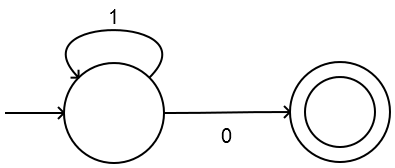
\includegraphics[scale=0.5]{DFAQ3.png}
    	\end{figure}
    	
    \section{Language}
    	The language of balanced parenthesis is not regular. 
    	To demonstrate it, let us consider a simplified version of the language 
    	where we consider only a sequence of k left parenthesis followed by
    	a sequence of k right parenthesis, this simplified version forming
    	a subset of the language we wish to prove irregular :
    	\newline
    	$$\{(^k )^k\}$$
    	
    	Using pumping lemmas, we can easily prove this language irregular by defining 
    	$w = \{(^k )^k\}$. By the pumping lemma, there should be some decomposition 
    	w = xyz with $|xy| \le p$ and $|y| \ge 1$ such that $x(y^i)z$ 
    	in L for every $i \ge 0$. \newline
    	
    	Since $|xy| \le p$, we know that y can only contain a non-null sequence of 
    	left parenthesis. This means that by pumping y and obtaining $xy^2 z$, we will
    	a sequence of parenthesis with more open parenthesis than closed parenthesis.
    	\newline
    	
    	Thus, this sequence will never be part of our simplified language L, and since
    	this subset of the original language cannot be represent by a regular expression,
    	we can infer that the whole language similarly cannot be represented.

\end{document}
